\chapter{Information Extraction}


One important the problem of this system is how to build the models from Job Description and Resume. The first step of model generating is information extraction. Both resumes and job descriptions are written in natural language, so we need to extract information from such un-structured or semi-structured data source, and transfer them to some designed structure.

\section{Text Processing Pipeline}

One important problem of this system is how to extract models from Job Descriptions and Resumes.
In Nature Language Processing, especially in Information Extraction, pipeline is a well adopted architecture~\cite{sarawagi2008information}. This architecture will also be used in this system to extract models of job openings and candidate's resumes. The system will process the job opening in the following steps, which is shown in Figure~\ref{fig:Pipeline}:

\begin{enumerate}
    \item HTML parser will parse the job description web pages that are obtained from web scrawler. It will get the HTML element that contains the main content of the job description.
    \item Segment module will separate the job description into paragraphs according to HTML tags at first, then separate each paragraph into sentences.
    \item The sentences will be tokenized as string array, and sent to the Classification module. Classification module will determine the category of the sentence, and mark the category of the sentence.
    \item Preprocessing module will delete unreadable characters, normalize some spelling tokens in the sentence.
    \item Annotation module will annotate the tokens with sematic and ontology labels. The sentences will be transferred to multi-layered data structure.
    \item The layered sentences will be matched with pre-defined patterns. If any pattern could be matched, the ontology information will be stored in the job model.
    \item After every sentence has be processed in the pipeline, the job model will be stored into database.
\end{enumerate}


\begin{figure}[htbp]
  \centering
  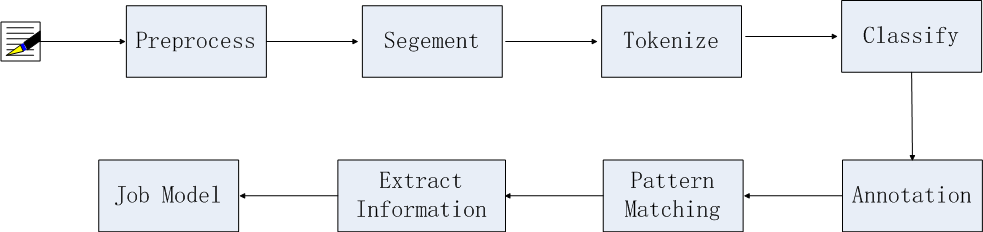
\includegraphics[scale=0.4]{images/pipeline.png}
  \caption{Job Description Process Pipeline}
  \label{fig:Pipeline}
\end{figure}


\section{Machine learning and Rule-based IE technologies}

Chiticariu et al. \cite{chiticariu2013rule}summarized the pros and cons of machine learning (ML) and rule-based IE technologies in Table

\begin{table}[ht]
\caption{Pros and Cons of ML and Rule-Based IE technologies } % title of Table
\centering % used for centering table
\begin{tabular}{ | c |  p{6cm} | p{6cm} | } % centered columns (4 columns)

\hline  %inserts double horizontal lines
 & Pros  & Cons  \\ [0.5ex] % inserts table
%heading
\hline % inserts single horizontal line
Rule-based &
    \begin{singlespace}
       \textbullet~Declarative  \par
       \textbullet~Easy to comprehend  \par
       \textbullet~Easy to maintain\par
       \textbullet~Easy to incorporate domain knowledge\par
       \textbullet~Easy to trace and fix the cause of errors  \par
    \end{singlespace}
    &  \begin{singlespace}
      \textbullet~Heuristic \par
       \textbullet~Requires tedious manual labor \par
       \end{singlespace}  \\
\hline
ML-based &
    \begin{singlespace}
       \textbullet~Trainable  \par
       \textbullet~Adaptable \par
       \textbullet~Reduces manual effort \par
    \end{singlespace}
    &  \begin{singlespace}
      \textbullet~Requires labeled data \par
       \textbullet~Requires retraining  for domain adaptation \par
        \textbullet~Requires ML expertise  to use or maintain \par
       \textbullet~Opaque  \par
       \end{singlespace} \\
\hline %inserts single line
\end{tabular}
\label{tab:mlrb} % is used to refer this table in the text
\end{table}

In this work, we prefer the rule-based approach because: 
\begin{enumerate}
    \item Most of sentences that contain the information we needed followed some common pattern.
    \item Lots of sentences are not grammatical correct, some of them missing subject, some of them are just a list of skills. 
    \item Processing speed is also a big concern, rule-based pattern matching is faster. 
\end{enumerate}



\section{Semantic Label}



After labeling, we could use some hybrid pattern like:
We don't need to match the real words in the sentence, or first level of semantic label, we could just match the high level semantic label.


\begin{table}[ht]
\caption{Labeled sentence } % title of Table
\centering % used for centering table
\begin{tabular}{   | c | c | c | c |c | c |c | c | c |  }
 \hline
     DE LEVEL   & DEGREE & IN & MAJOR            & OR & MAJOR  &.  \\
 \hline
     BS LEVEL   & DEGREE & IN & MAJOR CS         & OR & MAJOR INFO & .      \\
 \hline
    bachelors   & degree & in & computer science & or & information systems & .     \\
  \hline
\end{tabular}
\label{tab:labeldsent} % is used to refer this table in the text\section{Pipeline of Information Extraction}
\end{table}

\section{Pattern Matching}

Chang et al. presented cascaded regular expressions over tokens~\cite{chang2014tokensregex}, which defined a cascaded patterns over token sequences.

We proposed a more flexible regular expression over tokens framework.
One conception always have similar but different expression, like Bachelor's degree, in job description it could be written into bachelors degree, B.S., 4 years degree, and so on. IN this work, we annotate words in the sentence with semantic label. 